\begin{figure}

\center
\begin{comment}
python3 CounterfactualModel_Remington_VIZ.py 0 0 10.0 400 10000 UNIFORM UNIMODAL2 4567   
python3 CounterfactualModel_Remington_VIZ.py 1 0 10.0 400 10000 UNIFORM UNIMODAL2 4567   
python3 CounterfactualModel_Remington_VIZ.py 2 0 10.0 400 10000 UNIFORM UNIMODAL2 4567   
python3 CounterfactualModel_Remington_VIZ.py 4 0 10.0 400 10000 UNIFORM UNIMODAL2 4567   
python3 CounterfactualModel_Remington_VIZ.py 6 0 10.0 400 10000 UNIFORM UNIMODAL2 4567   
python3 CounterfactualModel_Remington_VIZ.py 8 0 10.0 400 10000 UNIFORM UNIMODAL2 4567   


python3 RunSynthetic_DenseRemington_FreeEncoding_Zero_OnSim_OtherNoiseLevels_VarySize_Round2_VIZ.py 0  0 10.0 400 SimulateSynthetic2_DenseRemington_OtherNoiseLevels_VarySize.py_400_0_4567_N40000_UNIFORM_UNIMODAL2.txt
python3 RunSynthetic_DenseRemington_FreeEncoding_L1_OnSim_OtherNoiseLevels_VarySize_VIZ.py 1  0 10.0 400 SimulateSynthetic2_DenseRemington_OtherNoiseLevels_VarySize.py_400_1_4567_N40000_UNIFORM_UNIMODAL2.txt
python3 RunSynthetic_DenseRemington_FreeEncoding_OnSim_OtherNoiseLevels_VarySize_VIZ.py 2 0 10.0 400 SimulateSynthetic2_DenseRemington_OtherNoiseLevels_VarySize.py_400_2_4567_N40000_UNIFORM_UNIMODAL2.txt
python3 RunSynthetic_DenseRemington_FreeEncoding_OnSim_OtherNoiseLevels_VarySize_VIZ.py 4 0 10.0 400 SimulateSynthetic2_DenseRemington_OtherNoiseLevels_VarySize.py_400_4_4567_N40000_UNIFORM_UNIMODAL2.txt
python3 RunSynthetic_DenseRemington_FreeEncoding_OnSim_OtherNoiseLevels_VarySize_VIZ.py 6 0 10.0 400 SimulateSynthetic2_DenseRemington_OtherNoiseLevels_VarySize.py_400_6_4567_N40000_UNIFORM_UNIMODAL2.txt
python3 RunSynthetic_DenseRemington_FreeEncoding_OnSim_OtherNoiseLevels_VarySize_VIZ.py 8 0 10.0 400 SimulateSynthetic2_DenseRemington_OtherNoiseLevels_VarySize.py_400_8_4567_N40000_UNIFORM_UNIMODAL2.txt

python3 evaluateCrossValidationResults_Synthetic_DenseRemington.py SimulateSynthetic2_DenseRemington_OtherNoiseLevels_VarySize.py_400_0_4567_N40000_UNIFORM_UNIMODAL2.txt
python3 evaluateCrossValidationResults_Synthetic_DenseRemington.py SimulateSynthetic2_DenseRemington_OtherNoiseLevels_VarySize.py_400_1_4567_N40000_UNIFORM_UNIMODAL2.txt
python3 evaluateCrossValidationResults_Synthetic_DenseRemington.py SimulateSynthetic2_DenseRemington_OtherNoiseLevels_VarySize.py_400_2_4567_N40000_UNIFORM_UNIMODAL2.txt
python3 evaluateCrossValidationResults_Synthetic_DenseRemington.py SimulateSynthetic2_DenseRemington_OtherNoiseLevels_VarySize.py_400_4_4567_N40000_UNIFORM_UNIMODAL2.txt
python3 evaluateCrossValidationResults_Synthetic_DenseRemington.py SimulateSynthetic2_DenseRemington_OtherNoiseLevels_VarySize.py_400_6_4567_N40000_UNIFORM_UNIMODAL2.txt
python3 evaluateCrossValidationResults_Synthetic_DenseRemington.py SimulateSynthetic2_DenseRemington_OtherNoiseLevels_VarySize.py_400_8_4567_N40000_UNIFORM_UNIMODAL2.txt

\end{comment}

  \begin{minipage}[b]{0.45\linewidth}
    \centering


$p=0$

\sideimage{Original}{figures/CounterfactualModel_Remington_VIZ.py_4567_UNIFORM_UNIMODAL2_0_0_10.0_400.pdf}
\sideimage{Fitted}{figures/RunSynthetic_DenseRemington_FreeEncoding_Zero_OnSim_OtherNoiseLevels_VarySize_Round2_VIZ.py_SimulateSynthetic2_DenseRemington_OtherNoiseLevels_VarySize.py_400_0_4567_N40000_UNIFORM_UNIMODAL2.txt_0_0_10.0_400.pdf}

$p=1$

\sideimage{Original}{figures/CounterfactualModel_Remington_VIZ.py_4567_UNIFORM_UNIMODAL2_1_0_10.0_400.pdf}
\sideimage{Fitted}{figures/RunSynthetic_DenseRemington_FreeEncoding_L1_OnSim_OtherNoiseLevels_VarySize_VIZ.py_SimulateSynthetic2_DenseRemington_OtherNoiseLevels_VarySize.py_400_1_4567_N40000_UNIFORM_UNIMODAL2.txt_1_0_10.0_400.pdf}
%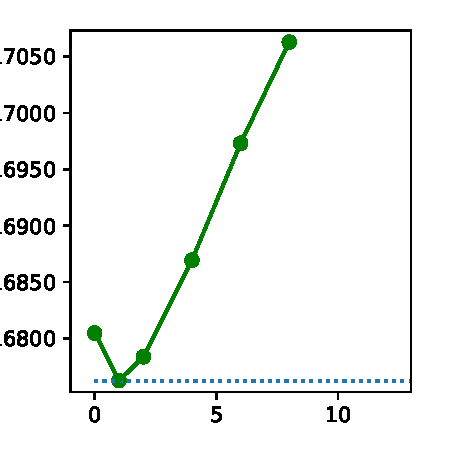
\includegraphics[width=0.15\textwidth]{figures/evaluateCrossValidationResults_Synthetic_DenseRemington.py_SimulateSynthetic2_DenseRemington_OtherNoiseLevels_VarySize.py_400_1_4567_N40000_UNIFORM_UNIMODAL2.txt.pdf}



$p=2$

\sideimage{Original}{figures/CounterfactualModel_Remington_VIZ.py_4567_UNIFORM_UNIMODAL2_2_0_10.0_400.pdf}

\sideimage{Fitted}{figures/RunSynthetic_DenseRemington_FreeEncoding_OnSim_OtherNoiseLevels_VarySize_VIZ.py_SimulateSynthetic2_DenseRemington_OtherNoiseLevels_VarySize.py_400_2_4567_N40000_UNIFORM_UNIMODAL2.txt_2_0_10.0_400.pdf}
%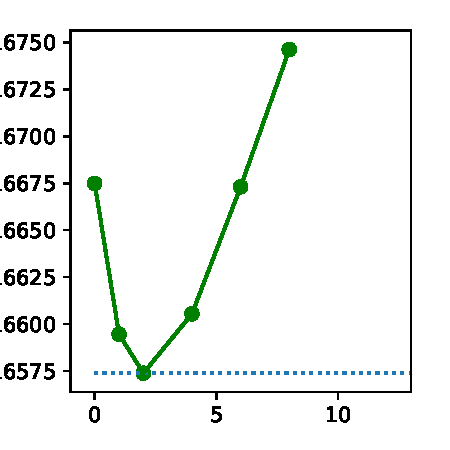
\includegraphics[width=0.15\textwidth]{figures/evaluateCrossValidationResults_Synthetic_DenseRemington.py_SimulateSynthetic2_DenseRemington_OtherNoiseLevels_VarySize.py_400_2_4567_N40000_UNIFORM_UNIMODAL2.txt.pdf}


  \end{minipage}%
  \hfill
  \begin{minipage}[b]{0.45\linewidth}
    \centering


$p=4$

\sideimage{Original}{figures/CounterfactualModel_Remington_VIZ.py_4567_UNIFORM_UNIMODAL2_2_0_10.0_400.pdf}

\sideimage{Fitted}{figures/RunSynthetic_DenseRemington_FreeEncoding_OnSim_OtherNoiseLevels_VarySize_VIZ.py_SimulateSynthetic2_DenseRemington_OtherNoiseLevels_VarySize.py_400_4_4567_N40000_UNIFORM_UNIMODAL2.txt_4_0_10.0_400.pdf}
%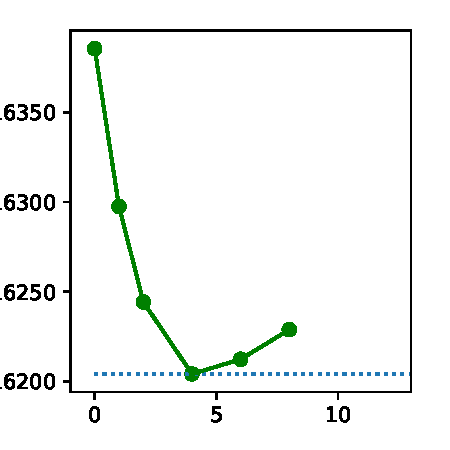
\includegraphics[width=0.15\textwidth]{figures/evaluateCrossValidationResults_Synthetic_DenseRemington.py_SimulateSynthetic2_DenseRemington_OtherNoiseLevels_VarySize.py_400_4_4567_N40000_UNIFORM_UNIMODAL2.txt.pdf}

$p=6$

\sideimage{Original}{figures/CounterfactualModel_Remington_VIZ.py_4567_UNIFORM_UNIMODAL2_2_0_10.0_400.pdf}

\sideimage{Fitted}{figures/RunSynthetic_DenseRemington_FreeEncoding_OnSim_OtherNoiseLevels_VarySize_VIZ.py_SimulateSynthetic2_DenseRemington_OtherNoiseLevels_VarySize.py_400_6_4567_N40000_UNIFORM_UNIMODAL2.txt_6_0_10.0_400.pdf}
%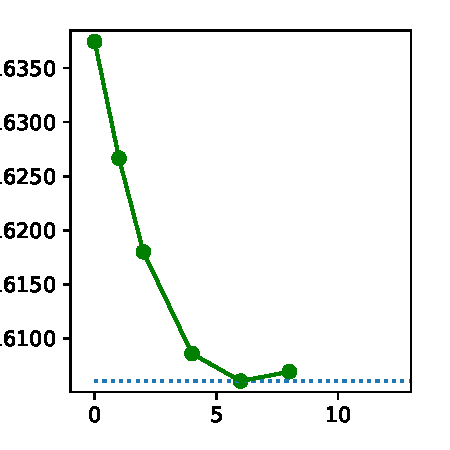
\includegraphics[width=0.15\textwidth]{figures/evaluateCrossValidationResults_Synthetic_DenseRemington.py_SimulateSynthetic2_DenseRemington_OtherNoiseLevels_VarySize.py_400_6_4567_N40000_UNIFORM_UNIMODAL2.txt.pdf}

$p=8$

\sideimage{Original}{figures/CounterfactualModel_Remington_VIZ.py_4567_UNIFORM_UNIMODAL2_2_0_10.0_400.pdf}

\sideimage{Fitted}{figures/RunSynthetic_DenseRemington_FreeEncoding_OnSim_OtherNoiseLevels_VarySize_VIZ.py_SimulateSynthetic2_DenseRemington_OtherNoiseLevels_VarySize.py_400_8_4567_N40000_UNIFORM_UNIMODAL2.txt_8_0_10.0_400.pdf}
%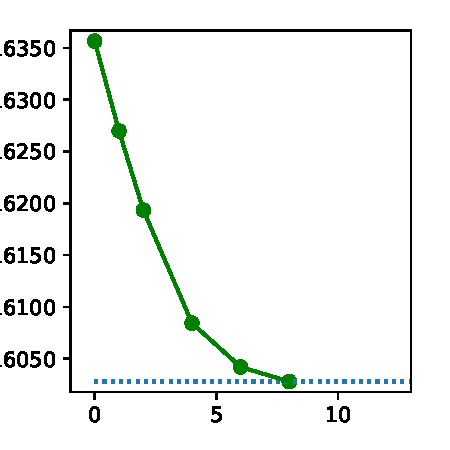
\includegraphics[width=0.15\textwidth]{figures/evaluateCrossValidationResults_Synthetic_DenseRemington.py_SimulateSynthetic2_DenseRemington_OtherNoiseLevels_VarySize.py_400_8_4567_N40000_UNIFORM_UNIMODAL2.txt.pdf}


\end{minipage}




\caption{
Interval Stimulus Space: Identifiability of encoding and prior (40K trials, 4 levels of sensory noise).
%While we here assume in fitting that the loss function is already known, results in Figure~\ref{fig:recover-loss-circ-uniform-periodic} show that the loss function is also largely identifiable in this situation.
We note that, in the vicinity of the boundary, the biases have an additional component, added to the attraction and repulsion terms in Equation 2 of the main paper, described formally in Theorem 3 of \citet{hahn2024unifying}.
See Section~\ref{sec:att-rep} for discussion of Attraction and Repulsion components.
}\label{fig:fit-uniform-unimodal}

\end{figure}


